\documentclass[ignorenonframetext,]{beamer}
\setbeamertemplate{caption}[numbered]
\setbeamertemplate{caption label separator}{: }
\setbeamercolor{caption name}{fg=normal text.fg}
\beamertemplatenavigationsymbolsempty
\usepackage{lmodern}
\usepackage{amssymb,amsmath}
\usepackage{ifxetex,ifluatex}
\usepackage{fixltx2e} % provides \textsubscript
\ifnum 0\ifxetex 1\fi\ifluatex 1\fi=0 % if pdftex
  \usepackage[T1]{fontenc}
  \usepackage[utf8]{inputenc}
\else % if luatex or xelatex
  \ifxetex
    \usepackage{mathspec}
  \else
    \usepackage{fontspec}
  \fi
  \defaultfontfeatures{Ligatures=TeX,Scale=MatchLowercase}
\fi
\usetheme[]{AnnArbor}
\usecolortheme{dolphin}
\usefonttheme{structuresmallcapsserif}
% use upquote if available, for straight quotes in verbatim environments
\IfFileExists{upquote.sty}{\usepackage{upquote}}{}
% use microtype if available
\IfFileExists{microtype.sty}{%
\usepackage{microtype}
\UseMicrotypeSet[protrusion]{basicmath} % disable protrusion for tt fonts
}{}
\newif\ifbibliography
\hypersetup{
            pdftitle={Diff-in-Diff and Fixed Effects},
            pdfauthor={Annie Chen},
            pdfborder={0 0 0},
            breaklinks=true}
\urlstyle{same}  % don't use monospace font for urls
\usepackage{color}
\usepackage{fancyvrb}
\newcommand{\VerbBar}{|}
\newcommand{\VERB}{\Verb[commandchars=\\\{\}]}
\DefineVerbatimEnvironment{Highlighting}{Verbatim}{commandchars=\\\{\}}
% Add ',fontsize=\small' for more characters per line
\usepackage{framed}
\definecolor{shadecolor}{RGB}{248,248,248}
\newenvironment{Shaded}{\begin{snugshade}}{\end{snugshade}}
\newcommand{\KeywordTok}[1]{\textcolor[rgb]{0.13,0.29,0.53}{\textbf{#1}}}
\newcommand{\DataTypeTok}[1]{\textcolor[rgb]{0.13,0.29,0.53}{#1}}
\newcommand{\DecValTok}[1]{\textcolor[rgb]{0.00,0.00,0.81}{#1}}
\newcommand{\BaseNTok}[1]{\textcolor[rgb]{0.00,0.00,0.81}{#1}}
\newcommand{\FloatTok}[1]{\textcolor[rgb]{0.00,0.00,0.81}{#1}}
\newcommand{\ConstantTok}[1]{\textcolor[rgb]{0.00,0.00,0.00}{#1}}
\newcommand{\CharTok}[1]{\textcolor[rgb]{0.31,0.60,0.02}{#1}}
\newcommand{\SpecialCharTok}[1]{\textcolor[rgb]{0.00,0.00,0.00}{#1}}
\newcommand{\StringTok}[1]{\textcolor[rgb]{0.31,0.60,0.02}{#1}}
\newcommand{\VerbatimStringTok}[1]{\textcolor[rgb]{0.31,0.60,0.02}{#1}}
\newcommand{\SpecialStringTok}[1]{\textcolor[rgb]{0.31,0.60,0.02}{#1}}
\newcommand{\ImportTok}[1]{#1}
\newcommand{\CommentTok}[1]{\textcolor[rgb]{0.56,0.35,0.01}{\textit{#1}}}
\newcommand{\DocumentationTok}[1]{\textcolor[rgb]{0.56,0.35,0.01}{\textbf{\textit{#1}}}}
\newcommand{\AnnotationTok}[1]{\textcolor[rgb]{0.56,0.35,0.01}{\textbf{\textit{#1}}}}
\newcommand{\CommentVarTok}[1]{\textcolor[rgb]{0.56,0.35,0.01}{\textbf{\textit{#1}}}}
\newcommand{\OtherTok}[1]{\textcolor[rgb]{0.56,0.35,0.01}{#1}}
\newcommand{\FunctionTok}[1]{\textcolor[rgb]{0.00,0.00,0.00}{#1}}
\newcommand{\VariableTok}[1]{\textcolor[rgb]{0.00,0.00,0.00}{#1}}
\newcommand{\ControlFlowTok}[1]{\textcolor[rgb]{0.13,0.29,0.53}{\textbf{#1}}}
\newcommand{\OperatorTok}[1]{\textcolor[rgb]{0.81,0.36,0.00}{\textbf{#1}}}
\newcommand{\BuiltInTok}[1]{#1}
\newcommand{\ExtensionTok}[1]{#1}
\newcommand{\PreprocessorTok}[1]{\textcolor[rgb]{0.56,0.35,0.01}{\textit{#1}}}
\newcommand{\AttributeTok}[1]{\textcolor[rgb]{0.77,0.63,0.00}{#1}}
\newcommand{\RegionMarkerTok}[1]{#1}
\newcommand{\InformationTok}[1]{\textcolor[rgb]{0.56,0.35,0.01}{\textbf{\textit{#1}}}}
\newcommand{\WarningTok}[1]{\textcolor[rgb]{0.56,0.35,0.01}{\textbf{\textit{#1}}}}
\newcommand{\AlertTok}[1]{\textcolor[rgb]{0.94,0.16,0.16}{#1}}
\newcommand{\ErrorTok}[1]{\textcolor[rgb]{0.64,0.00,0.00}{\textbf{#1}}}
\newcommand{\NormalTok}[1]{#1}

% Prevent slide breaks in the middle of a paragraph:
\widowpenalties 1 10000
\raggedbottom

\AtBeginPart{
  \let\insertpartnumber\relax
  \let\partname\relax
  \frame{\partpage}
}
\AtBeginSection{
  \ifbibliography
  \else
    \let\insertsectionnumber\relax
    \let\sectionname\relax
    \frame{\sectionpage}
  \fi
}
\AtBeginSubsection{
  \let\insertsubsectionnumber\relax
  \let\subsectionname\relax
  \frame{\subsectionpage}
}

\setlength{\parindent}{0pt}
\setlength{\parskip}{6pt plus 2pt minus 1pt}
\setlength{\emergencystretch}{3em}  % prevent overfull lines
\providecommand{\tightlist}{%
  \setlength{\itemsep}{0pt}\setlength{\parskip}{0pt}}
\setcounter{secnumdepth}{0}
\usepackage{multirow}
\usepackage{graphicx}
\graphicspath{ {./images/} }
\DeclareUnicodeCharacter{2212}{-}
\newcommand{\indep}{\rotatebox[origin=c]{90}{$\models$}}

\title{Diff-in-Diff and Fixed Effects}
\author{Annie Chen}
\date{February 12, 2020}

\begin{document}
\frame{\titlepage}

\begin{frame}[fragile]{Pset 5}

\begin{itemize}[<+->]
\tightlist
\item
  \texttt{R} code for plotting effect of observed covariates
\end{itemize}

\end{frame}

\begin{frame}{Review of D-i-D}

Fill in the blanks:

\begin{center}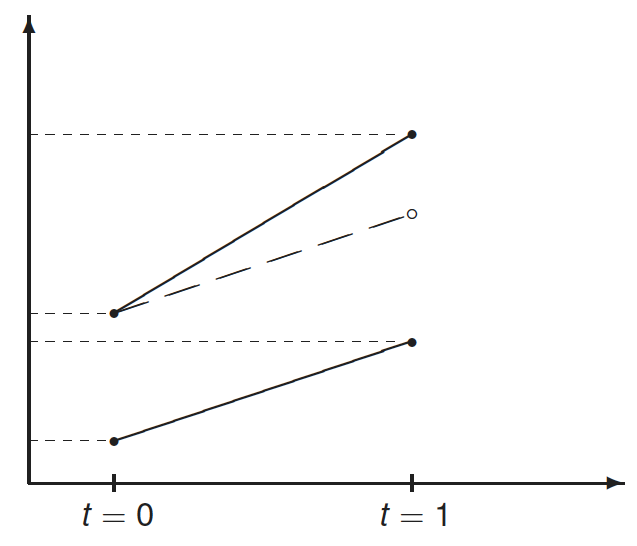
\includegraphics[width=0.6\linewidth]{d-i-d_graph2} \end{center}

\end{frame}

\begin{frame}{Review of D-i-D}

\begin{itemize}[<+->]
\tightlist
\item
  What is the causal estimand in a D-i-D?

  \begin{itemize}[<+->]
  \tightlist
  \item
    The ATT in the post-treatment period:
    \(\mathbb{E}[Y_{i1}(1) - Y_{i1}(0) | D_i = 1]\)
  \end{itemize}
\end{itemize}

\end{frame}

\begin{frame}{D-i-D Estimation with Regression}

\[Y_{it} = \alpha + \beta_1Treated_{i} + \beta_2Period_{t} + \beta_3(Treated_i \times Period_t) + u_{it}\]

\begin{itemize}[<+->]
\item
  \(\beta_1\) captures pre-existing differences between treated and
  control while \(\beta_2\) is the change over time common to both
  groups.
\item
  Same as two-way fixed effects? What happens in D-i-D model if I
  include both unit and time FE?
  \[Y_{it} = \alpha + \delta_i + \tau_t + \beta_3(Treated_{i} \times Period_{t}) + u_{it}\]
\end{itemize}

\end{frame}

\begin{frame}[fragile]{Voter Graditude Example (Bectel and Hainmueller.
2011)}

\begin{itemize}[<+->]
\item
  Unit of analysis is electoral districts.
\item
  Treatment is \texttt{Flooded}, a binary variable indicating whether an
  electoral district was directly affected by the 2002
  flood.\footnote<.->{Federal elections are set exogenously by the
    German Constitution.}
\item
  The dependent variable is the SPD PR vote share for a given electoral
  district.\footnote<.->{Models 4, 7, and 10 are the first-differenced
    DID regressions with the DV as the change in vote share between two
    election periods.}
\end{itemize}

\end{frame}

\begin{frame}{}

\begin{itemize}[<+->]
\item
  Interested in
  \(\mathbb{E}[Y_{i1, 2002} | D_i = 1] - \mathbb{E}[Y_{i0, 2002} | D_i = 1]\)
\item
  \color{black}{Assume}
  \color{blue}{$E[Y_{0i, 2002} - Y_{0i, 1998}|D_{i} = 1] = E[Y_{0i, 2002} - Y_{0i, 1998}|D_{i} = 0]$}

  \begin{itemize}[<+->]
  \tightlist
  \item
    \color{black}{Read: "In the absence of the flood, the average SPD vote share in the affected districts would have followed a similar trend as the average SPD vote share in unaffected districts."}
  \end{itemize}
\item
  \(\hat{Y}_{it} = \hat{\nu}_{i} + \hat{\delta}_{t} + \hat{\beta}D_{it} + X_{it}^{T}\hat{\alpha} + \hat{\epsilon}_{it}\)

  \begin{itemize}[<+->]
  \tightlist
  \item
    where \(\hat{\nu}_{i}\) and \(\hat{\delta}_{t}\) are district and
    time fixed effects respectively.
  \end{itemize}
\end{itemize}

\end{frame}

\begin{frame}[fragile]{}

\begin{itemize}[<+->]
\tightlist
\item
  \texttt{Flooded} and \texttt{PostPeriod} are equivalent to the
  interaction between Treatment and Period (Treatment = 1 are flooded
  districts and Period = 1 is post-treatment)
\end{itemize}

\small

\begin{Shaded}
\begin{Highlighting}[]
\NormalTok{all_data }\OperatorTok\StringTok{ }
\StringTok{  }\KeywordTok{filter}\NormalTok{(data_period }\OperatorTok{==}\StringTok{ "1998–2002"}\NormalTok{) }\OperatorTok\StringTok{ }
\StringTok{  }\NormalTok{dplyr}\OperatorTok{::}\KeywordTok{select}\NormalTok{(}\KeywordTok{c}\NormalTok{(}\StringTok{"wkr"}\NormalTok{, }\StringTok{"year"}\NormalTok{, }\StringTok{"spd_z_vs"}\NormalTok{, }
                  \StringTok{"Flooded"}\NormalTok{, }\StringTok{"PostPeriod"}\NormalTok{)) }\OperatorTok\StringTok{ }
\StringTok{  }\KeywordTok{head}\NormalTok{()}
\end{Highlighting}
\end{Shaded}

\begin{verbatim}
## # A tibble: 6 x 5
##     wkr  year spd_z_vs Flooded PostPeriod
##   <dbl> <dbl>    <dbl>   <dbl>      <dbl>
## 1     1  1998     47.2       0          0
## 2     1  2002     44.0       0          1
## 3     2  1998     43.5       0          0
## 4     2  2002     42.4       0          1
## 5     3  1998     44.6       0          0
## 6     3  2002     41.2       0          1
\end{verbatim}

\normalsize

\end{frame}

\begin{frame}[fragile]{First-Difference Estimator}

\(\Delta Y_{it} = \beta \Delta D_{it} + \Delta u_{it}\) (first, without
covariates)

\begin{Shaded}
\begin{Highlighting}[]
\KeywordTok{library}\NormalTok{(plm)}
\NormalTok{fd_mod <-}\StringTok{ }\NormalTok{all_data }\OperatorTok\StringTok{ }
\StringTok{  }\KeywordTok{filter}\NormalTok{(data_period }\OperatorTok{==}\StringTok{ "1998–2002"}\NormalTok{) }\OperatorTok\StringTok{ }
\StringTok{  }\KeywordTok{plm}\NormalTok{(}\DataTypeTok{data =}\NormalTok{ ., }\DataTypeTok{index =} \KeywordTok{c}\NormalTok{(}\StringTok{"wkr"}\NormalTok{), }
      \DataTypeTok{model =} \StringTok{"fd"}\NormalTok{, }\CommentTok{# first difference estimator}
      \DataTypeTok{formula =}\NormalTok{ spd_z_vs }\OperatorTok{~}\StringTok{ }\NormalTok{Flooded }\OperatorTok{*}\StringTok{ }\NormalTok{PostPeriod)}
\end{Highlighting}
\end{Shaded}

\end{frame}

\begin{frame}[fragile]{First-Difference Estimator}

\tiny

\begin{verbatim}
## Oneway (individual) effect First-Difference Model
## 
## Call:
## plm(formula = spd_z_vs ~ Flooded * PostPeriod, data = ., model = "fd", 
##     index = c("wkr"))
## 
## Balanced Panel: n = 299, T = 2, N = 598
## Observations used in estimation: 299
## 
## Residuals:
##      Min.   1st Qu.    Median   3rd Qu.      Max. 
## -11.97010  -1.50274  -0.12258   1.24436  11.77026 
## 
## Coefficients: (1 dropped because of singularities)
##             Estimate Std. Error t-value  Pr(>|t|)    
## (Intercept) -2.88037    0.22058 -13.058 < 2.2e-16 ***
## Flooded      7.14401    0.70827  10.087 < 2.2e-16 ***
## ---
## Signif. codes:  0 '***' 0.001 '**' 0.01 '*' 0.05 '.' 0.1 ' ' 1
## 
## Total Sum of Squares:    5238.1
## Residual Sum of Squares: 3901.6
## R-Squared:      0.25515
## Adj. R-Squared: 0.25265
## F-statistic: 101.74 on 1 and 297 DF, p-value: < 2.22e-16
\end{verbatim}

\normalsize

\end{frame}

\begin{frame}[fragile]{Correcting Standard Errors}

\begin{Shaded}
\begin{Highlighting}[]
\CommentTok{# this does not support twoway clustering... }
\KeywordTok{coeftest}\NormalTok{(fd_mod, }\DataTypeTok{vcov. =} \KeywordTok{vcovHC}\NormalTok{(fd_mod, }\DataTypeTok{type =} \StringTok{"HC2"}\NormalTok{, }
                                \DataTypeTok{cluster =} \StringTok{"group"}\NormalTok{))}
\end{Highlighting}
\end{Shaded}

\begin{verbatim}
## 
## t test of coefficients:
## 
##             Estimate Std. Error t value  Pr(>|t|)    
## (Intercept) -2.88037    0.22758 -12.656 < 2.2e-16 ***
## Flooded      7.14401    0.47313  15.099 < 2.2e-16 ***
## ---
## Signif. codes:  0 '***' 0.001 '**' 0.01 '*' 0.05 '.' 0.1 ' ' 1
\end{verbatim}

\end{frame}

\begin{frame}[fragile]{Fixed Effects via Demeaning}

\(\tilde{Y}_{i} = \beta \tilde{D}_{i} + \tilde{u}_{i}\)

\small

\begin{Shaded}
\begin{Highlighting}[]
\NormalTok{all_data }\OperatorTok\StringTok{ }
\StringTok{  }\KeywordTok{filter}\NormalTok{(data_period }\OperatorTok{==}\StringTok{ "1998–2002"}\NormalTok{) }\OperatorTok\StringTok{ }
\StringTok{  }\KeywordTok{plm}\NormalTok{(}\DataTypeTok{data =}\NormalTok{ ., }\DataTypeTok{index =} \KeywordTok{c}\NormalTok{(}\StringTok{"wkr"}\NormalTok{, }\StringTok{"PostPeriod"}\NormalTok{), }
      \DataTypeTok{model =} \StringTok{"within"}\NormalTok{, }\CommentTok{# within estimator }
      \DataTypeTok{formula =}\NormalTok{ spd_z_vs }\OperatorTok{~}\StringTok{ }\NormalTok{Flooded }\OperatorTok{*}\StringTok{ }\NormalTok{PostPeriod) }\OperatorTok\StringTok{ }
\StringTok{  }\KeywordTok{coeftest}\NormalTok{(., }\DataTypeTok{vcov. =} \KeywordTok{vcovHC}\NormalTok{(., }\DataTypeTok{type=}\StringTok{"HC2"}\NormalTok{))}
\end{Highlighting}
\end{Shaded}

\begin{verbatim}
## 
## t test of coefficients:
## 
##             Estimate Std. Error t value  Pr(>|t|)    
## Flooded      7.14401    0.46983  15.206 < 2.2e-16 ***
## PostPeriod1 -2.88037    0.22737 -12.668 < 2.2e-16 ***
## ---
## Signif. codes:  0 '***' 0.001 '**' 0.01 '*' 0.05 '.' 0.1 ' ' 1
\end{verbatim}

\normalsize

\begin{itemize}[<+->]
\tightlist
\item
  When \(T = 2\), demeaning and first-difference estimators are
  equivalent!
\end{itemize}

\end{frame}

\begin{frame}[fragile]{Including covariates}

\begin{itemize}[<+->]
\item
  Exercise: Carefully select covariates (\(\textbf{X}_{it}\)) and
  reestimate the new model including these covariates:
  \(\hat{Y}_{it} = \hat{\nu}_{i} + \hat{\delta}_{t} + \hat{\beta}D_{it} + X_{it}^{T}\hat{\alpha} + \hat{\epsilon}_{it}\).
\item
  Assume that these are all \_ \_ \_ - \_ \_ \_ \_ \_ \_ \_ \_ \_
  covariates.
\end{itemize}

\begin{Shaded}
\begin{Highlighting}[]
\NormalTok{all_data }\OperatorTok\StringTok{ }
\StringTok{  }\NormalTok{dplyr}\OperatorTok{::}\KeywordTok{select}\NormalTok{(}\KeywordTok{starts_with}\NormalTok{(}\StringTok{"xx"}\NormalTok{)) }\OperatorTok\StringTok{ }
\StringTok{  }\KeywordTok{colnames}\NormalTok{()}
\end{Highlighting}
\end{Shaded}

\begin{verbatim}
##  [1] "xxsinc_SPD"        "xxpopdensity_"     "xxshpop_o60_"     
##  [4] "xxpopnetinp1000_"  "xxue_"             "xxshagric_"       
##  [7] "xxshmanu_"         "xxshtradservice_"  "xxshotherservice_"
## [10] "xxshforeign_"
\end{verbatim}

\end{frame}

\begin{frame}[fragile]{Including covariates}

\small

\begin{Shaded}
\begin{Highlighting}[]
\NormalTok{form_covars <-}\StringTok{ }\NormalTok{spd_z_vs }\OperatorTok{~}\StringTok{ }\NormalTok{Flooded }\OperatorTok{*}\StringTok{ }\NormalTok{PostPeriod }\OperatorTok{+}
\StringTok{                  }\CommentTok{# controls}
\StringTok{                  }\NormalTok{xxpopdensity_ }\OperatorTok{+}\StringTok{ }\CommentTok{# share pop density}
\StringTok{                  }\NormalTok{xxshpop_o60_ }\OperatorTok{+}\StringTok{ }\CommentTok{# share pop over 60}
\StringTok{                  }\NormalTok{xxpopnetinp1000_ }\OperatorTok{+}\StringTok{ }\CommentTok{# share pop outflow}
\StringTok{                  }\NormalTok{xxue_ }\OperatorTok{+}\StringTok{ }\CommentTok{# unemployment}
\StringTok{                  }\NormalTok{xxshagric_ }\OperatorTok{+}\StringTok{ }\CommentTok{# employment share (agriculture) }
\StringTok{                  }\NormalTok{xxshmanu_ }\OperatorTok{+}\StringTok{ }\CommentTok{# employment share (manufacturing)        }
\StringTok{                  }\NormalTok{xxshtradservice_ }\OperatorTok{+}\StringTok{ }\CommentTok{# employment share (trade) }
\StringTok{                  }\NormalTok{xxshotherservice_ }\OperatorTok{+}\StringTok{ }\CommentTok{# employment share (other services)}
\StringTok{                  }\NormalTok{xxshforeign_ }\OperatorTok{+}\CommentTok{# share of foreigners}
\StringTok{                  }\NormalTok{xxsinc_SPD }\CommentTok{# SPD incumbent in Land}
\end{Highlighting}
\end{Shaded}

\normalsize

\end{frame}

\begin{frame}[fragile]

\small

\begin{Shaded}
\begin{Highlighting}[]
\NormalTok{full_mod <-}\StringTok{ }\NormalTok{all_data }\OperatorTok\StringTok{ }
\StringTok{  }\KeywordTok{filter}\NormalTok{(data_period }\OperatorTok{==}\StringTok{ "1998–2002"}\NormalTok{) }\OperatorTok\StringTok{ }
\StringTok{  }\KeywordTok{plm}\NormalTok{(}\DataTypeTok{data =}\NormalTok{ ., }\DataTypeTok{index =} \KeywordTok{c}\NormalTok{(}\StringTok{"wkr"}\NormalTok{, }\StringTok{"PostPeriod"}\NormalTok{), }
      \DataTypeTok{model =} \StringTok{"within"}\NormalTok{, form_covars)}
\end{Highlighting}
\end{Shaded}

\normalsize

\tiny

\begin{table}
\begin{center}
\begin{tabular}{l c }
\hline
 & Model 1 \\
\hline
Flooded            & $6.91^{***}$  \\
                   & $(0.76)$      \\
PostPeriod1        & $-3.98^{***}$ \\
                   & $(0.69)$      \\
xxpopdensity\_     & $-0.06$       \\
                   & $(1.43)$      \\
xxshpop\_o60\_     & $0.40$        \\
                   & $(0.22)$      \\
xxpopnetinp1000\_  & $-0.04$       \\
                   & $(0.03)$      \\
xxue\_             & $-0.13$       \\
                   & $(0.16)$      \\
xxshagric\_        & $-1.58$       \\
                   & $(4.05)$      \\
xxshmanu\_         & $-1.20$       \\
                   & $(4.03)$      \\
xxshtradservice\_  & $-1.31$       \\
                   & $(4.02)$      \\
xxshotherservice\_ & $-1.12$       \\
                   & $(4.02)$      \\
xxshforeign\_      & $20.09$       \\
                   & $(21.33)$     \\
xxsinc\_SPD        & $-1.12$       \\
                   & $(0.63)$      \\
\hline
R$^2$              & 0.44          \\
Adj. R$^2$         & -0.16         \\
Num. obs.          & 598           \\
\hline
\multicolumn{2}{l}{\scriptsize{$^{***}p<0.001$, $^{**}p<0.01$, $^*p<0.05$}}
\end{tabular}
\caption{Statistical models}
\label{table:coefficients}
\end{center}
\end{table}

\normalsize

\end{frame}

\begin{frame}[fragile]{Parallel Trends Assumption}

\begin{itemize}[<+->]
\item
  \(\mathbb{E}[Y_{i1}(0) - Y_{i0}(0)| D_i = 1] = \mathbb{E}[Y_{i1}(0) - Y_{i0}(0)| D_i = 0]\)
\item
  Check \color{blue}{leads}\color{black}{: 1994 - 1998}
\end{itemize}

\begin{Shaded}
\begin{Highlighting}[]
\NormalTok{all_data }\OperatorTok\StringTok{ }
\StringTok{  }\KeywordTok{filter}\NormalTok{(data_period }\OperatorTok{==}\StringTok{ "1994–1998"}\NormalTok{) }\OperatorTok\StringTok{ }
\StringTok{  }\KeywordTok{plm}\NormalTok{(}\DataTypeTok{data =}\NormalTok{ ., }\DataTypeTok{index =} \KeywordTok{c}\NormalTok{(}\StringTok{"wkr"}\NormalTok{), }
    \DataTypeTok{model =} \StringTok{"fd"}\NormalTok{, }
    \DataTypeTok{formula =}\NormalTok{ spd_z_vs }\OperatorTok{~}\StringTok{ }\NormalTok{Flooded }\OperatorTok{*}\StringTok{ }\NormalTok{PostPeriod)}
\end{Highlighting}
\end{Shaded}

\begin{verbatim}
## 
## Model Formula: spd_z_vs ~ Flooded * PostPeriod
## <environment: 0x7fed44820078>
## 
## Coefficients:
## (Intercept)     Flooded 
##  4.61036210 -0.00040711
\end{verbatim}

\begin{itemize}[<+->]
\tightlist
\item
  The more pre-treatment periods the better!
\end{itemize}

\end{frame}

\begin{frame}{Visual Inspection of Parallel Trends Assumption}

\begin{center}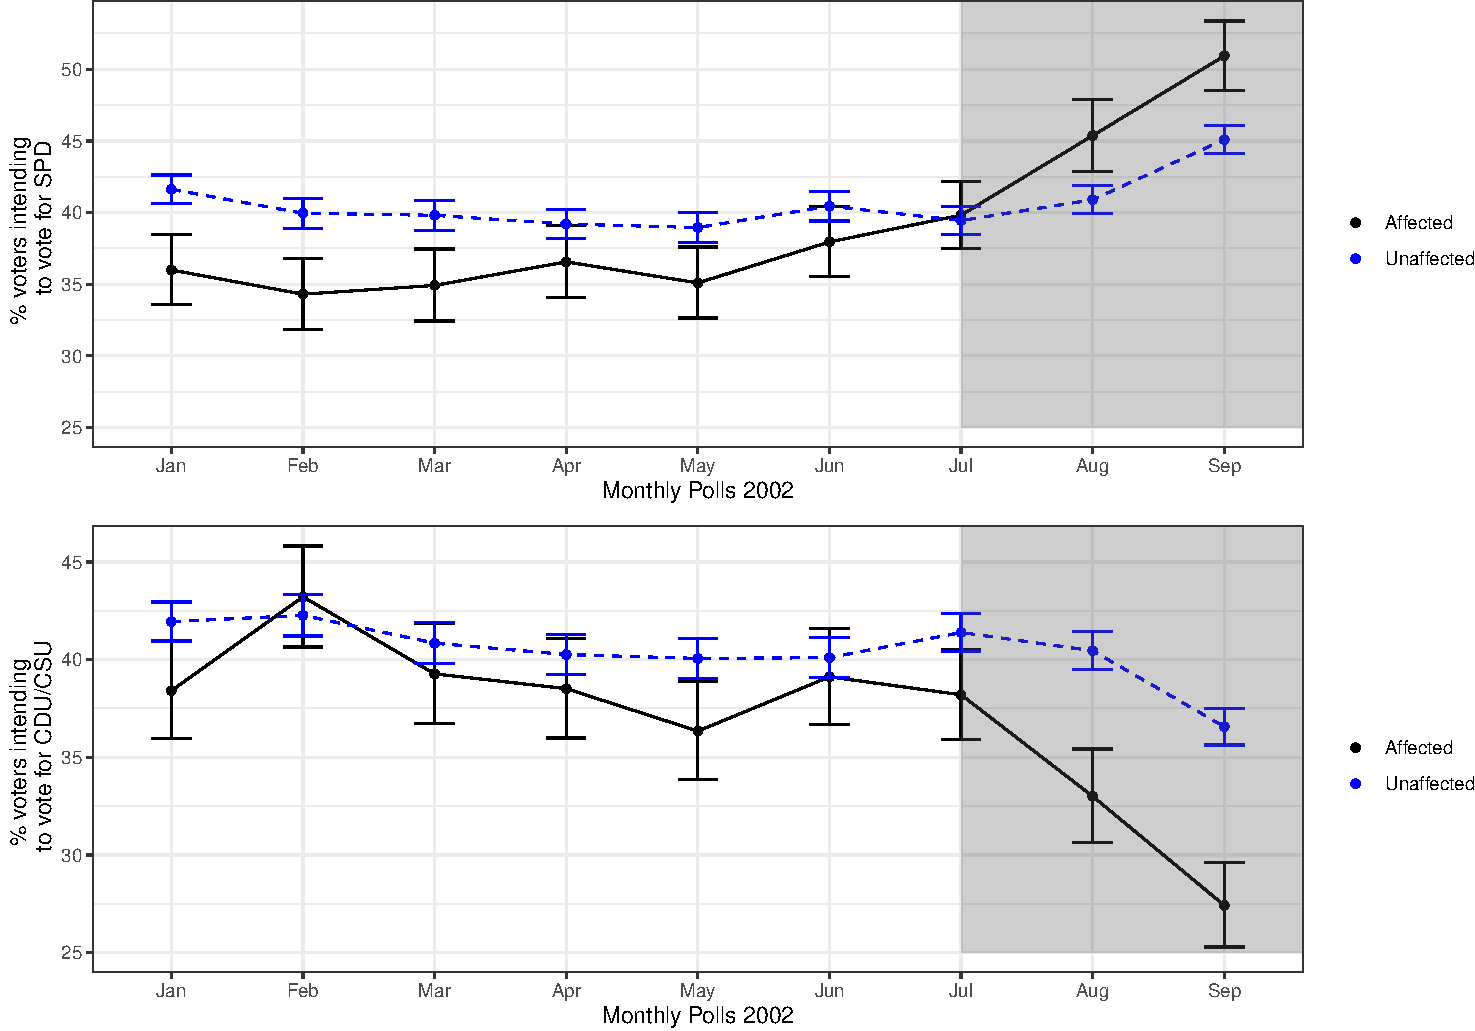
\includegraphics[width=0.8\linewidth]{Diff_in_diff_FEs_files/figure-beamer/unnamed-chunk-16-1} \end{center}

\end{frame}

\begin{frame}{More Diagnostics}

\begin{center}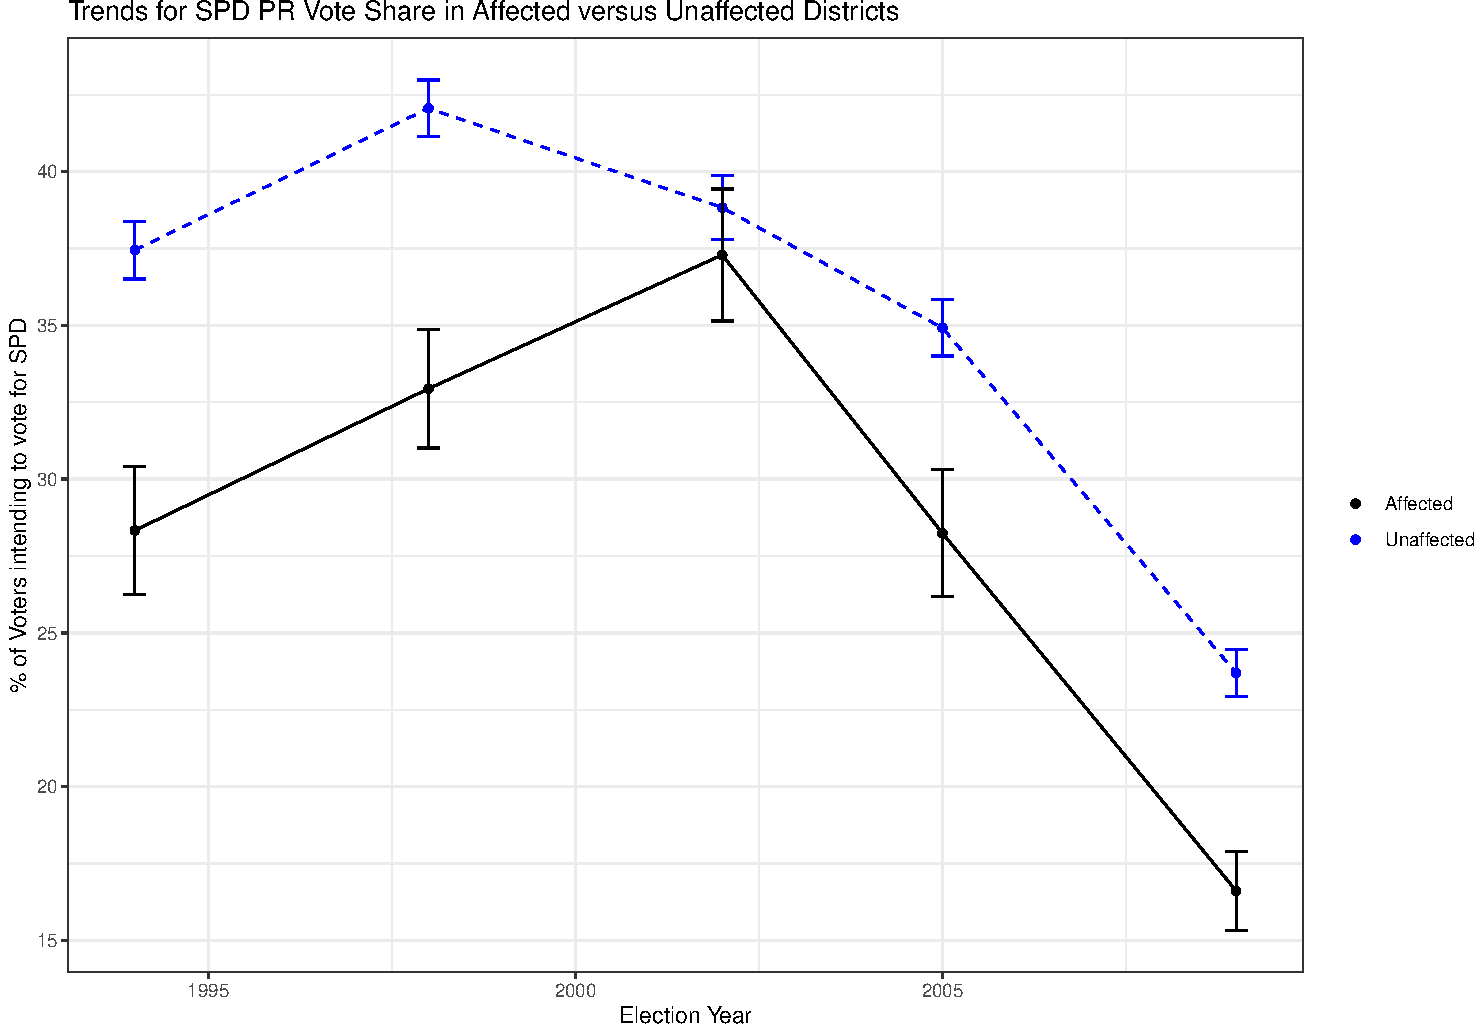
\includegraphics[width=0.8\linewidth]{Diff_in_diff_FEs_files/figure-beamer/unnamed-chunk-17-1} \end{center}

\end{frame}

\begin{frame}{Competing Explanations}

\begin{itemize}[<+->]
\tightlist
\item
  A competing hypothesis involves the possible confounding salience of
  the Iraq war issue during the 2009 campaign.
\end{itemize}

\begin{center}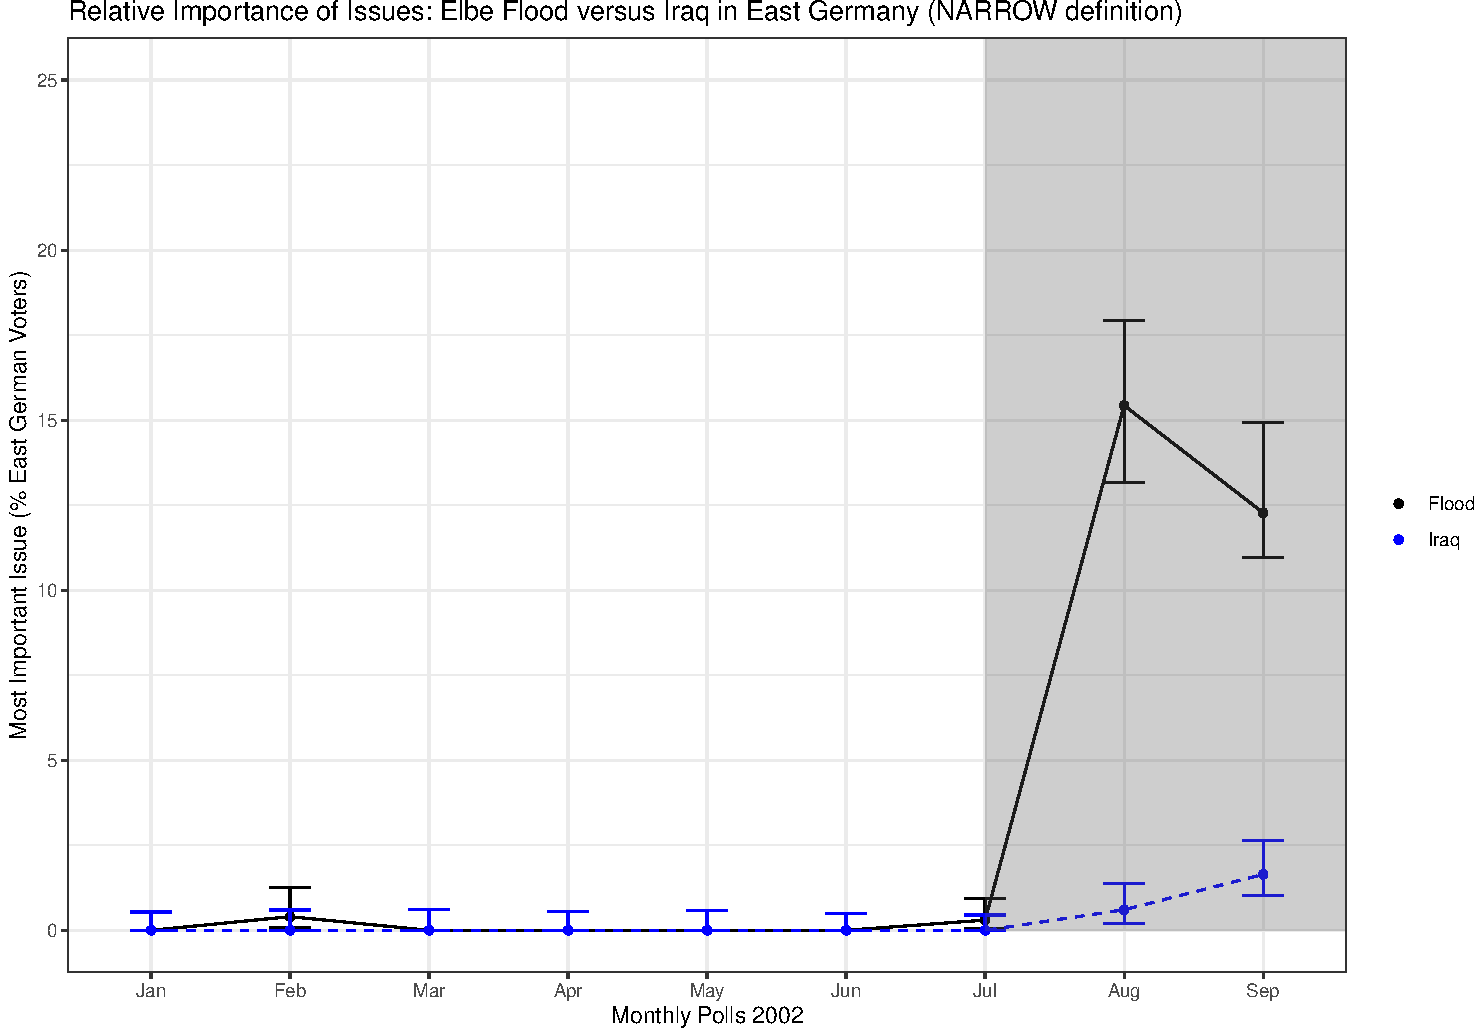
\includegraphics[width=0.7\linewidth]{Diff_in_diff_FEs_files/figure-beamer/unnamed-chunk-19-1} \end{center}

\end{frame}

\end{document}
